\documentclass[25pt, a0paper, portrait, margin=0mm, innermargin=15mm,%
colspace=15mm, subcolspace=8mm, blockverticalspace=15mm]{tikzposter}
\usepackage[utf8]{inputenc}
\usepackage[T1]{fontenc}
\usepackage[croatian]{babel}
\usepackage{csquotes}
\newcommand{\cmd}[1]{{\bf \color{violet}#1}} 

\tikzposterlatexaffectionproofon

\renewenvironment{tikzfigure}[1][]{
  \def \rememberparameter{#1}
  \vspace{10pt}
  \refstepcounter{figurecounter}
  \begin{center}
  }{
    \ifx\rememberparameter\@empty
    \else %nothing
    \\[10pt]
    {\small Slika~\thefigurecounter: \rememberparameter}
    \fi
  \end{center}
}

\begin{document}
\title{Kreiranje postera pomoću Ti\emph{k}Zpostera} 
\institute{PMF -- Matematički odsjek}
\author{Ivica Nakić} 
\usetheme{Envelope} 
\usecolorstyle[colorPalette=BlueGrayOrange]{Russia}
\usetitlestyle{VerticalShading}
\usenotestyle{VerticalShading}
\colorlet{notebgcolor}{brown!30}
\colorlet{titlebgcolor}{red!30}
\colorlet{titlefgcolor}{black!80}
\maketitle 

\begin{columns}
         \column{.55}
         \block[roundedcorners=40]{Zaglavlje \LaTeX{} dokumenta}{
             \begin{quote}
                 \cmd{\textbackslash documentclass[20pt, a0paper, portrait, margin=10mm, innermargin=15mm,
                 blockverticalspace=15mm, colspace=15mm, subcolspace=8mm]\{tikzposter\}\\
                 \textbackslash title\{Naslov\}\\
                 \textbackslash author\{Autor(i)\}\\
                 \textbackslash institute\{Institucija\}\\
                 \textbackslash titlegraphic\{Logo\}\\
                 \textbackslash begin\{document\}\\
                 \textbackslash maketitle}
             \\ \dots         \end{quote}
        Veličinu fonta možemo birati između veličina: \cmd{12pt}, \cmd{14pt}, \cmd{17pt}, \cmd{20pt}, \cmd{25pt}. Predefinirana veličina je \cmd{25pt}.
        
        Veličine papira koje možemo birati su: \cmd{a0paper}, \cmd{a1paper}, \cmd{a2paper}.

        Orijentacija je \cmd{portrait} ili \cmd{landscape}.

        \cmd{margin} definira razmak između ruba postera i ruba papira.

        \cmd{innermargin} definira razmak između ruba blokova i ruba postera.

        \cmd{colspace} definira horizontalni razmak između stupaca.

        \cmd{blockverticalspace} definira vertikalni razmak između blokova. 

        S naredbom \cmd{\textbackslash tikzposterlatexaffectionproofoff} odnosno \\
        \cmd{\textbackslash tikzposterlatexaffectionproofon} isključujemo odnosno isključujemo pojavljivanje informacije o tome kako je kreiran poster.

     }
     \note[targetoffsetx=-.05\textwidth,targetoffsety=11.5cm,innersep=.4cm,angle=-45,connection]{Opcionalni argumenti pri formatiranju postera.}
     \block{Naslov}{
         Naslov se kreira standardnom neredbom \cmd{\textbackslash maketitle[{\it opcije}]}, a u opcijama možete promijeniti relativno skaliranje naslova \cmd{titletextscale}, širinu \cmd{width}, razmak između naslova i vrha postera (\cmd{titletotopverticalspace}), razmak
         između (dna) naslova i ostatka postera (\cmd{titletoblockverticalspace}) te razmak između naslova i logoa (\cmd{titlegraphictotitleverticalspace}).

		Naredbom \cmd{\textbackslash settitle} se može posve promijeniti izgled naslova, više informacija se može naći u priručniku za Ti\emph{k}z\textbf{poster}.}
     \block{Blokovi}{
         Blokovi sa slažu u mrežu s predefiniranom širinom \cmd{\textbackslash textwdith}, dakle cijele stranice. Kreiraju se naredbom
         \begin{quote}
             \textbackslash\cmd{block[{\it opcije}]\{{\it naslov}\}\{{\it sadržaj}\}}
         \end{quote}
         Naslov nije nužan. Ostali blokovi se slažu ispod prethodnog, s razmakom definiranim s \cmd{blockverticalspace}.

         Pozicija bloka te naslova bloka se može promijeniti korištenjem opcija
         \begin{quote}
             \cmd{titleoffsetx, titleoffsety, bodyoffsetx, bodyoffsety}
         \end{quote}
         kojima se namješta vertikalna te horizonalna pozicija naslova bloka i samog bloka.
         Druga opcija je da se definira veličina obzirom na veličinu postera korišetenjem
         \begin{quote}
             \cmd{titlewidthscale, bodywidthscale}
         \end{quote}
         Pozicija naslova se može namjestiti pomoću \cmd{titleleft, titlecenter, titleright}, 
         a tijelo bloka se može namjestiti po visini pomoću \cmd{bodyverticalshift}. 
         Pomoću \cmd{roundedcorners, linewidth} mijenjamo oblik bloka. Unutarnje margine naslova bloka namiještaju se s \cmd{titleinnersep, bodyinnersep}.

          \innerblock[]{Unutrašnji blokovi}{Kreiraju se unutar blokova naredbom \textbackslash\cmd{innerblock[{\it opcije}]\{{\it Naslov}\}\{{\it Tekst}\}}. Opcije su analogne opcijama za \cmd{\textbackslash block}. }
            \coloredbox{Tekst možemo naglasiti tako da ga stavimo unutar obojanih kutija koristeći naredbu \textbackslash\cmd{coloredbox[{\it opcije}]\{{\it Tekst\}}}. Opcijama možemo promijeniti npr.\ širinu \cmd{width}, boju pozadine \cmd{bgclor}, boju teksta \cmd{fgcolor}.}
     }

    \block{Ostalo}{
 	         \begin{tikzfigure}[Grafika se ubacuje na standardni način, osim što se umjesto okoline \cmd{figure} koristi okolina \cmd{tikzfigure}.]
			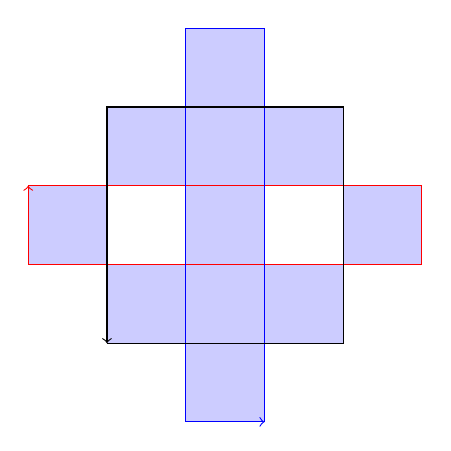
\begin{tikzpicture}[fill=blue!20] 
			\fill (0,2) -- (0,3) -- (5,3) -- (5,2) 
				  (2,0) -- (3,0) -- (3,5) -- (2,5)
				  (1,1) -- (4,1) -- (4,4) -- (1,4); 
			\draw[red,->]
			(0,3) -- (5,3) -- (5,2) -- (0,2) -- (0,3); 
			\draw[blue,->]
			(3,0) -- (3,5) -- (2,5) -- (2,0) -- (3,0); 
			\draw[->]
			(1,1) -- (4,1) -- (4,4) -- (1,4) -- (1,1); 
			\end{tikzpicture} 
         \end{tikzfigure}   

    }    

     \note[targetoffsetx=10cm, targetoffsety=1cm,rotate=1,angle=270,radius=10cm,width=.75\textwidth,innersep=.4cm]{
     Bilješke se mogu \enquote{vezati} za prethodni blok naredbom
     \begin{quote} \cmd{\textbackslash note[{\it opcije}]\{{\it sadržaj}\}}\end{quote}
     Bilješke se predefinirano smještaju malo udesno od središta prethodnog bloka, te se mogu povezati s blokom koristeći opciju \cmd{connection}.  

    Bilješka se može pomaknuti pomoću \cmd{targetoffsetx, targetoffsety}, rotirati pomoću \cmd{rotate}, i mijenjati širinu s \cmd{width}.  
    Smještaj bilješke (s obzirom na blok) je dan u polarnim koordinatama \cmd{ radius, angle}. 
    Bilješka je \textbf{uvijek} nacrtana iznad drugog teksta.
    }
     \column{.45}
         \block{Stupci}{
              Ako ne želimo imati blokove u samo jednom stupcu, možemo koristiti okolinu \cmd{columns} koja se koristi i kod prezentacija. Na primjer, k\^od
             \begin{quote}
                 \cmd{\noindent \textbackslash begin\{columns\}\\
                 \textbackslash column\{.6\}\\
                 \textbackslash block\{\dots\}\{\dots\}\\
                 \textbackslash column\{.4\}\\
                 \textbackslash block\{\dots\}\{\dots\}\\
                 \textbackslash block\{\dots\}\{\dots\}\\
                 \textbackslash end\{columns\}
                 }
             \end{quote}
             će kreirati dva stupca širina 60\% i 40\% ukupne širine, s razmakom između stupaca definiranom s
             \cmd{colspace}. Širinu možemo zadati i eksplicitno. 
         }

         \begin{subcolumns}
             \subcolumn{.45}
             \block{Podstupci}{Za dodatnu podjelu možemo koristiti \cmd{subcolumns} okolinu. Princip je isti kao i kod \cmd{columns} okoline, samo je širina relativna s obzirom na širinu stupca.}

             \subcolumn{.5}
             \block{}{Jedan primjer:
                 \begin{quote}
                     \cmd{\textbackslash begin\{subcolumns\}\\
                     \textbackslash subcolumn\{.6\}\\
                     \textbackslash block\{\dots\}\{\dots\}\\
                     \textbackslash subcolumn\{.4\}\\
                     \textbackslash block\{\dots\}\{\dots\}\\
                     \textbackslash block\{\dots\}\{\dots\}\\
                     \textbackslash end\{subcolumns\}
                     }
             \end{quote}
         }
         \end{subcolumns}

         \block[titlewidthscale=.8,bodywidthscale=.85,titleoffsety=9.5mm,bodyoffsety=9mm]{Mijenjanje izgleda postera}{
         	Izgled postera, uključujući izgled naslova, pozadinu, izgled blokova i bilješki se može jednostavno promijeniti promijenom teme 
         	  \begin{quote}
                 \cmd{\textbackslash usetheme\{{\em ime teme}\}}.
             \end{quote}
             Predefinirane teme su: Default, Rays, Basic, Simple, Envelope, Wave, Board, Autumn, Desert. Možemo i sami definirati svoju temu.

             Možemo mijenjati i samo dio izgleda naredbama
             \begin{quote}
                 \cmd{\textbackslash usebackgroundstyle[]\{\}, \textbackslash usetitlestyle[]\{\},\\ \textbackslash useblockstyle[]\{\},\textbackslash innerblockstyle[]\{\},\\ \textbackslash usenotestyle[]\{\}}
             \end{quote}
             Možemo mijenjati i stil te paletu boja pomoću	
             \begin{quote}
                 \cmd{\textbackslash usecolorstyle[colorPalette=\emph{paleta boja}]\{{\emph{stil boja}\}}}
             \end{quote}
             Predefinirani stilovi:
             \begin{description}
             	\item[Pozadina] Default, VerticalGradation, Rays, BottomVerticalGradation, Empty.
             	\item[Naslov] Default, Basic, Empty, Filled, Envelope, Wave, VerticalShading.
             	\item[Blok] Default, Basic, Minimal, Envelope, Corner, Slide, TornOut.
             	\item[Unutrašnji blok] Default i Table te ostali stilovi za blokove.  
             	\item[Bilješka] Default, VerticalShading, Corner, Sticky.
             	\item[Paleta boja] Default, BlueGrayOrange, GreenGrayViolet, PurpleGrayBlue, BrownBlueOrange.
             	\item[Stil boja] Default, Australia, Britain, Sweden, Spain, Russia, Denmark, Germany.  
             \end{description}
            Možemo i sami kreirati stilove za pojedine dijelove postera. 
          }
     \block[titlewidthscale=.8,bodywidthscale=.85,titleoffsety=9.5mm,bodyoffsety=9mm]{Primjer definiranja stila boja}{
    \begin{quote}	
    \cmd{	 
    \textbackslash definecolorstyle\{KolorStil\} \{ \\
	\textbackslash definecolor\{bojaJedan\}\{named\}\{blue\} \\
	\textbackslash definecolor\{bojaDva\}\{named\}\{yellow\} \\
	\textbackslash definecolor\{bojaTri\}\{named\}\{orange\} \\
	\}\{ \\
	\textbackslash colorlet\{backgroundcolor\}\{bojaJedan\} \\
	\textbackslash colorlet\{framecolor\}\{black\}	\\ 
	\textbackslash colorlet\{titlefgcolor\}\{black\} \\
	\textbackslash colorlet\{titlebgcolor\}\{bojaJedan\} \\
	\textbackslash colorlet\{blocktitlebgcolor\}\{bojaTri\} \\
	\}
	}
	\end{quote}
     }

     \end{columns}

\end{document}